\documentclass[a4paper,12pt]{report}
%\documentclass[a4paper,11pt,twoside]{./Systems/StyleThese}
%\documentclass[11pt]{book}
% %\usepackage[final]{pdfpages}										% pour intgrer un PDF dans le document
% \usepackage{eurosym}
% \usepackage{amsmath,amssymb}             % AMS Math
% %%AQUI\usepackage[frenchb]{babel}
% \usepackage[latin1]{inputenc}
% \usepackage[T1]{fontenc}
% \usepackage[left=1.5in,right=1.3in,top=1.1in,bottom=1.1in,includefoot,includehead,headheight=13.6pt]{geometry}
% \usepackage{tabularx}
% \usepackage{epsfig, amssymb,graphicx,latexsym}
% \usepackage{moreverb} %% pour le verbatim en boite
% \usepackage{multirow} %% pour regrouper un texte sur plusieurs lignes dans une table
% \usepackage{url} %% pour citer les url par \url
% \usepackage[all]{xy} %% pour la barre au dessus des symboles
% \usepackage{Systems/shorttoc} %% pour plusieurs tables des matires par la commande
% \usepackage{textcomp} %% pour le symbol pour mille par \textperthousand.
% \usepackage{zed-csp}

\renewcommand{\baselinestretch}{1.05}

%changement de police
\renewcommand\familydefault{bch}

% Table of contents for each chapter
\usepackage[nottoc, notlof, notlot]{tocbibind}
% \usepackage[french]{minitoc}
% \setcounter{minitocdepth}{2}
% \mtcindent=15pt
% 
% \newcommand{\minitocNewPage}{\minitoc\newpage}
% \mtcsetfont{minitoc}{section}{\normalfont\small}
% \mtcsetfont{minitoc}{subsection}{\normalfont\small}
% \mtcsetfont{minitoc}{subsubsection}{\normalfont\small}

% Use \minitoc where to put a table of contents
% Use \minitocNewPage where to put a table of contents with a new page behind

\usepackage{aecompl}

% Glossary / list of abbreviations

\usepackage[intoc]{nomencl}
\renewcommand{\nomname}{Liste des Abr�viations}

\makenomenclature

% My pdf code

\usepackage{ifpdf}

\ifpdf
  \usepackage[pdftex]{graphicx}
  \DeclareGraphicsExtensions{.jpg}
  \usepackage[a4paper,pagebackref,hyperindex=true]{hyperref}
\else
  \usepackage{graphicx}
  \DeclareGraphicsExtensions{.ps,.eps, .jpg}
  \usepackage[a4paper,dvipdfm,pagebackref,hyperindex=true]{hyperref}
\fi

\graphicspath{{.}{images/}}

% Links in pdf
\usepackage{color}
\definecolor{linkcol}{rgb}{0,0,0.4} 
\definecolor{citecol}{rgb}{0.5,0,0} 

% Change this to change the informations included in the pdf file

\hypersetup
{
bookmarksopen=true,
pdftitle="",  %titre document
pdfauthor="", %auteur du document
pdfsubject="", %sujet du document
%pdftoolbar=false, %barre d'outils non visible
pdfmenubar=true, %barre de menu visible
pdfhighlight=/O, %effet d'un clic sur un lien hypertexte
colorlinks=true, %couleurs sur les liens hypertextes
pdfpagemode=UseNone, %aucun mode de page
pdfpagelayout=SinglePage, %ouverture en simple page
pdffitwindow=true, %pages ouvertes entierement dans toute la fenetre
linkcolor=linkcol, %couleur des liens hypertextes internes
citecolor=citecol, %couleur des liens pour les citations
urlcolor=linkcol %couleur des liens pour les url
}

% definitions.
% -------------------

\setcounter{secnumdepth}{3}
\setcounter{tocdepth}{2}

% Some useful commands and shortcut for maths:  partial derivative and stuff

\newcommand{\pd}[2]{\frac{\partial #1}{\partial #2}}
\def\abs{\operatorname{abs}}
\def\argmax{\operatornamewithlimits{arg\,max}}
\def\argmin{\operatornamewithlimits{arg\,min}}
\def\diag{\operatorname{Diag}}
\newcommand{\eqRef}[1]{(\ref{#1})}

\usepackage{rotating}                    % Sideways of figures & tables
%\usepackage{bibunits}
%\usepackage[sectionbib]{chapterbib}          % Cross-reference package (Natural BiB)
%\usepackage{natbib}                  % Put References at the end of each chapter
                                         % Do not put 'sectionbib' option here.
                                         % Sectionbib option in 'natbib' will do.
\usepackage{fancyhdr}                    % Fancy Header and Footer

% \usepackage{txfonts}                     % Public Times New Roman text & math font
  
%%% Fancy Header %%%%%%%%%%%%%%%%%%%%%%%%%%%%%%%%%%%%%%%%%%%%%%%%%%%%%%%%%%%%%%%%%%
% Fancy Header Style Options

\pagestyle{fancy}                       % Sets fancy header and footer
\fancyfoot{}                            % Delete current footer settings

%\renewcommand{\chaptermark}[1]{         % Lower Case Chapter marker style
%  \markboth{\chaptername\ \thechapter.\ #1}}{}} %

%\renewcommand{\sectionmark}[1]{         % Lower case Section marker style
%  \markright{\thesection.\ #1}}         %

\fancyhead[LE,RO]{\bfseries\thepage}    % Page number (boldface) in left on even
% pages and right on odd pages
\fancyhead[RE]{\bfseries\nouppercase{\leftmark}}      % Chapter in the right on even pages
\fancyhead[LO]{\bfseries\nouppercase{\rightmark}}     % Section in the left on odd pages

\let\headruleORIG\headrule
\renewcommand{\headrule}{\color{black} \headruleORIG}
\renewcommand{\headrulewidth}{1.0pt}
\usepackage{colortbl}
\arrayrulecolor{black}

\fancypagestyle{plain}{
  \fancyhead{}
  \fancyfoot{}
  \renewcommand{\headrulewidth}{0pt}
}

%AQUI \usepackage{./Systems/MyAlgorithm}
%AQUI \usepackage[noend]{./Systems/MyAlgorithmic}

%%% Clear Header %%%%%%%%%%%%%%%%%%%%%%%%%%%%%%%%%%%%%%%%%%%%%%%%%%%%%%%%%%%%%%%%%%
% Clear Header Style on the Last Empty Odd pages
\makeatletter

\def\cleardoublepage{\clearpage\if@twoside \ifodd\c@page\else%
  \hbox{}%
  \thispagestyle{empty}%              % Empty header styles
  \newpage%
  \if@twocolumn\hbox{}\newpage\fi\fi\fi}

\makeatother
 
%%%%%%%%%%%%%%%%%%%%%%%%%%%%%%%%%%%%%%%%%%%%%%%%%%%%%%%%%%%%%%%%%%%%%%%%%%%%%%% 
% Prints your review date and 'Draft Version' (From Josullvn, CS, CMU)
\newcommand{\reviewtimetoday}[2]{\special{!userdict begin
    /bop-hook{gsave 20 710 translate 45 rotate 0.8 setgray
      /Times-Roman findfont 12 scalefont setfont 0 0   moveto (#1) show
      0 -12 moveto (#2) show grestore}def end}}
% You can turn on or off this option.
% \reviewtimetoday{\today}{Draft Version}
%%%%%%%%%%%%%%%%%%%%%%%%%%%%%%%%%%%%%%%%%%%%%%%%%%%%%%%%%%%%%%%%%%%%%%%%%%%%%%% 

\newenvironment{maxime}[1]
{
\vspace*{0cm}
\hfill
\begin{minipage}{0.5\textwidth}%
%\rule[0.5ex]{\textwidth}{0.1mm}\\%
\hrulefill $\:$ {\bf #1}\\
%\vspace*{-0.25cm}
\it 
}%
{%

\hrulefill
\vspace*{0.5cm}%
\end{minipage}
}

\let\minitocORIG\minitoc
%\renewcommand{\minitoc}{\minitocORIG \vspace{1.5em}}

\usepackage{multirow}
\usepackage{slashbox}

\newenvironment{bulletList}%
{ \begin{list}%
	{$\bullet$}%
	{\setlength{\labelwidth}{25pt}%
	 \setlength{\leftmargin}{30pt}%
	 \setlength{\itemsep}{\parsep}}}%
{ \end{list} }

\newtheorem{definition}{D�finition}
\renewcommand{\epsilon}{\varepsilon}

% centered page environment

\newenvironment{vcenterpage}
{\newpage\vspace*{\fill}\thispagestyle{empty}\renewcommand{\headrulewidth}{0pt}}
{\vspace*{\fill}}


\usepackage[latin1]{inputenc}% accent standard clavier
%\usepackage[frenchb]{babel}
%\usepackage[cyr]{aeguill}
%\usepackage[T1]{fontenc}
\usepackage{lmodern} 
\usepackage[]{graphicx}
\usepackage{amsmath}
\usepackage{amssymb}
\usepackage{tabularx}
\usepackage{epsfig,amsthm}
\usepackage{moreverb}
\usepackage{multirow}
\usepackage{url}
\usepackage[all]{xy}
\usepackage{./Systems/shorttoc}
\usepackage{./Systems/floatflt}
\usepackage{textcomp}

%\usepackage[lined,algonl,boxed]{./Systems/algorithm2e}
\usepackage[french,ruled,vlined]{./Systems/algorithm2e}
\usepackage{url}
%\SetKw{KwOr}{or}

\newtheorem{lemma}{Lemme}
\newtheorem{property}{Propri�t�}
%\newtheorem{definition}{Definition}
\newtheorem{remark}{Remarque}
\newtheorem{theorem}{Th�or�me}
\newtheorem{prop}{Proposition}
\renewcommand{\proof}{\textbf{Preuve}}
%\usepackage{cite}
\usepackage[]{natbib}
\usepackage{longtable}

\setcounter{secnumdepth}{3}
\setcounter{tocdepth}{3}

\usepackage{multicol}

%%%%  macro dans le pr�ambule %%%%
\makeatletter
\def\captionof#1#2{{\def\@captype{#1}#2}}
\makeatother
%%%% fin macro %%%%
%\begin{minipage}[b]{0.45\linewidth}


\usepackage{setspace}
%\doublespacing

\newcommand{\og}{\resizebox{5pt}{5pt}{$<\!<$}\ }
\newcommand{\fg}{\resizebox{5pt}{5pt}{$>\!>$}\ }
\newcommand{\quotefr}[1]{\resizebox{5pt}{5pt}{$<\!<$}\ {#1}\ \resizebox{5pt}{5pt}{$>\!>$}}

\makeindex
\def\underscore{\char`\_}

%\setlength{\doublerulesep}{\arrayrulewidth}

%==========================================================================================================
\begin{document}

%\addtocounter{page}{-1}
%------------------------------------------------------------------------------------------------------
%  Page de garde
\title{Application d'optimisation\\
Conception g�n�rale}
%\subtitle{Conception g�n�rale}
\author{J.C. Cr�put}
\date{Janvier 2015}
\maketitle


%------------------------------------------------------------------------------------------------------
%  Table des matieres
%\addcontentsline{toc}{chapter}{Introduction G�n�rale}
\markboth{Contents}{Introduction}
\tableofcontents

%==========================================================================================================

%  Chapitres
\chapter*{Introduction}
\label{intro_generale}
 \addcontentsline{toc}{chapter}{Introduction}
 \markboth{Introduction}{Introduction}
 
Ce document r�pond � une probl�matique d'optimisation type. La solution logicielle r�pond aux sp�cifications fournies dans le document :
\begin{itemize}
\item 		\textit{cahier\_des\_charges.pdf}
\end{itemize}

Le probl�me d'optimisation trait� est un pro\-bl�me NP-difficile fictif, trait� par m�ta-heuristique. La tr�s grande combinatoire du probl�me et l'�tude des approches d'optimisation de la litt�rature en recherche op�ra\-tionnelle am�ne � consid�rer son traitement par l'usage des m�thodes m�taheuristiques. Ce document pr�sente une solution type pour r�soudre le probl�me. La m�thode est bas�e sur des m�taheu\-ristiques de type recherche locale et algorithme �volu\-tionnaire et m�m�tique.

Les diff�rentes sections sont organis�es pour faire ressortir les principaux composants et �tapes de la conception et mod�lisation de l'algorithme d'opti\-misation et son implantation en C++. Les chapitres pr�sentent successivement les �l�ments suivants :
\begin{itemize}
\item 		\textit{D�finition du probl�me d'optimisation}
\item 		\textit{Principe de r�solution}
\item 		\textit{Structures de donn�es}
\item 		\textit{Op�rateurs de base}
\item 		\textit{Algorithme m�taheuristique}
\item 		\textit{Jeux de tests et �valuation}
\end{itemize}

Une conclusion g�n�rale termine le document.

\chapter{D�finition du probl�me d'optimisation}
\label{chapitre_2}

Le probl�me est apparent� au probl�me de fl�t optique (\textit{optical flow}).

Ici, nous donnons la d�finition du probl�me d'optimisation, ce qui revient � pr�ciser ses entr�es, ses sorties, et les contraintes et objectifs du probl�me.

\section{Entr�e/sortie du programme d'optimisation}
\label{entrees}

\begin{figure}[h]
\centering
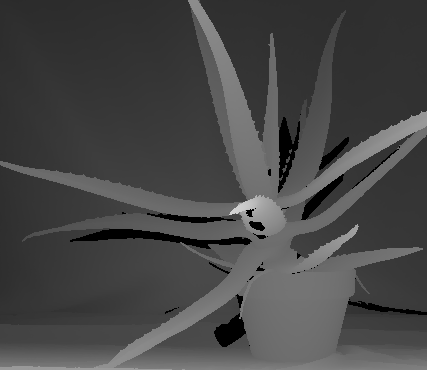
\includegraphics[width=5cm]{./Img/test_gd.png}
\caption{Entr�e : exemple d'entr�e}
\label{figure:entree}
\end{figure}

Le programme d'optimisation est une fonction d'optimisation qui transforme une donn�e d'entr�e en une solution de sortie, en principe optimale au sens des contraintes et objectifs du probl�me. La donn�e d'entr�e est pr�sent�e par la figure \ref{figure:entree}. Elle comporte diff�rents �l�ments. Un exemple de solution est donn� � la figure \ref{figure:solution}.

\begin{figure}[h]
\centering
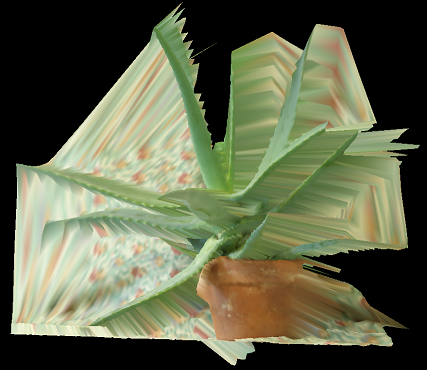
\includegraphics[width=5cm]{./Img/test.png}
\caption{Sortie : exemple de solution}
\label{figure:solution}
\end{figure}

\section{Fonction objectif}
\subsection{Fonction objectif globale agr�gative}

La fonction objectif globale � minimiser est une somme pond�r�e des objectifs d�finissant les crit�res et contraintes du probl�me :\\
\\
    $objectif ~=~ f\_objectif\_1~*~weightObjective1\\
            +~ f\_objectif\_2 ~*~ weightObjective2\\
            +~ f\_objectif\_3 ~*~ weightObjective3$
\\

La fonction objectif globale est r�alis�e par la fonction C++ :

\begin{itemize}
\item 		\textit{double SolutionObject::computeObjectif(void)}
\end{itemize}

Les diff�rents objectifs et crit�res sont pr�cis�s dans les sections suivantes.

\subsection{Objectif 1}

\subsection{Objectif 2}

\subsection{Objectif 3}

\section{D�finition du probl�me d'optimisation}

Le probl�me d'optimisation est d�fini par une entr�e, l'instance du probl�me, et une sortie, la solution du probl�me, dont l'�valuation doit correspondre � une valeur minimum de la fonction objectif agr�gative.

Une instance du probl�me consiste en diff�rents composants. La solution fournit des valeurs des variables du probl�me. Le but est de fournir une solution optimale au sens de la minimisation de la fonction objectif agr�gative.

Une solution est dite admissible lorsque toutes les contraintes sont satisfaites. La satisfaction d'une contrainte revient � une mise � 0 de certains objectifs.


\chapter{Approche d'optimisation}
\label{chapitre_resolution}

Les probl�mes de fl�t optique avec contraintes sont NP-difficiles. Nous n'avons pas trouv�, dans la litt�rature sur le sujet, de m�thode de r�solution exacte de ce type de probl�me r�pondant � nos besoins. Une instance avec tr�s peu d'�l�ments comporte d�j� une combinatoire de type factorielle qui rend tr�s difficile la r�solution exacte en temps raisonnable. Il para�t justifi� de tenter de r�soudre le probl�me par des m�thodes heuristiques et m�taheu\-ristiques. Dans ce cas, nous ne garantissons pas l'obtention syst�matique d'un optimum global, ce qui prendrait un temps infiniment long, mais nous cherchons des solutions admissibles et de bonne qualit� en temps raisonnable. Pour v�rifier l'efficacit�, les performances sont valid�es exp�rimentalement sur des jeux de tests repr�sentatifs du probl�me concret. Nous abordons dans ce chapitre la pr�sentation des principes de base des m�thodes m�ta\-heuristiques propos�es. 

\section{Strat�gie d'optimisation}
\label{strategies}

La d�marche de r�solution, appel�e aussi strat�gie de recherche ou d'optimi\-sation, est une d�marche heuristique, fond�e sur le principe des recherches locales d'une part, et sur le principe des algorithmes � base de population de solutions, tels que les algorithmes �volu\-tionnaires, d'autre part.

De mani�re imag�e, il s'agit de faire �voluer pas � pas une solution de d�part, tr�s approximative et ne respectant pas n�cessairement les contraintes, vers une solution admissible satisfaisant toutes les contraintes du probl�me, via des s�quences de mouvements simples et op�rations de \textit{swap}, plus ou moins al�atoires, portant sur les composants de la solution. Ces mouvements sont r�alis�s conjointement aux r��valuations rapides des valeurs des objectifs impact�s. Ce sont ces �valuations qui d�terminent et orientent la s�lection des mouvements r�alis�s.

Chaque mouvement de base de la solution comporte l'�valuation des objectifs li�s au composant consid�r�, le mouvement proprement dit, puis l'�valuation de l'impact du mouvement sur les valeurs des objectifs. Si l'impact est favorable, la nouvelle solution est retenue comme candidate � de nouvelles modifications, sinon elle n'est pas consid�r�e et la solution pr�c�dente est � nouveau utilis�e comme point de d�part ou pivot de la recherche locale.

La recherche locale met en oeuvre une d�marche d'optimisation par r�it�ration de mouvements locaux via les op�rateurs de base de la r�solution. Un des inconv�nients de la recherche locale r�side dans le minimum local o� elle peut se trouver lorsque les mouvements de faible amplitude ne sont pas suffisants � faire �voluer favorablement la solution. La r�ponse apport�e ici r�side, ou bien dans la r�it�ration du processus d'optimisation � partir de solutions al�atoires initiales diff�rentes, ou bien dans l'utilisation d'une d�marche �volu\-tionnaire m�m�tique.

Le principe informel de l'algorithme �volutionnaire m�m�tique consiste � appliquer des recherches locales sur une population de solutions, d'autres op�rations �ventuelles, et � proc�der � des s�lections et remplacements de solutions. Les solutions les moins satisfaisantes sont remplac�es par les plus satisfaisantes, � chaque it�ration, appel�e une g�n�ration. La meilleure solution produite est fournie en sortie.

Dans cette section, nous ne donnons que le principe g�n�ral des m�thodes sans entrer dans le d�tail des algorithmes. Les op�rateurs de base ainsi que les pseudo-codes des m�thodes de recherche sont pr�sent�s en d�tail dans les chapitres suivants. 

\section{Principe de la recherche locale}
\label{prin_local_search}
La recherche locale consiste en une modification locale d'une solution cou\-rante en consid�rant un voisinage plus ou moins large de cette solution. Cette solution courante, pas n�cessai\-rement admissible (satisfaisant toutes les contraintes), est obtenue au d�part par une m�thode de construction rapide. Les modifications locales d�terminent une intensification de la recherche dans une zone plus ou moins restreinte de l'espace des solutions. La r�i\-t�ration de la recherche locale � partir de solutions initiales al�atoires permet de diversifier la recherche \citep{johnson:97}. 

En se basant sur une solution de d�part pr�alablement construite mais pas n�cessaire\-ment admissible, trois versions de la strat�gie de recherche locale sont consid�r�es. La premi�re version est une m�thode de recherche al�atoire it�r�e, de type marche al�atoire, que nous appelons IRS, pour \textit{Iterated Random searh}. La deuxi�me est une m�thode de recherche locale gloutonne de type premier-meilleur que nous appelons ILS-FI, pour \textit{Iterated Local Search First Improvement}. La troisi�me est une recherche locale en profondeur que nous appelons ILS BI pour \textit{Iterated Local Search Best Improvement}. 

La m�thode IRS fait �voluer une solution courante en effectuant un nombre donn� de mouvements successifs dans le voisinage, ex�cut�s via un op�rateur de voisinage, puis s�lectionne la meilleure solution rencontr�e. Chaque solution examin�e est obtenue par modification de la solution pr�c�\-dente � l'aide de l'op�rateur de voisinage. Une suite de modifications de la solution courante est ex�cut�e, leur nombre �tant pr�alablement fix�. La meilleure solution rencontr�e est s�lectionn�e. Le proc�d� complet est r�it�r� un certain nombre de fois apr�s permutation �ventuelle des �pures pour favoriser l'�mergence d'un ordre valide de chargement. La m�thode est tr�s simple puisque tr�s peu d'op�rations de copie de donn�es sont effectu�es � chaque d'it�ration.

Dans les recherches locales ILS-FI et ILS-BI, une solution donn�e constitue l'�l�ment pivot autour duquel est effectu�e la recherche dans le voisinage. Chaque nouvelle solution examin�e est obtenue par modification de la solution pivot avec l'op�rateur de voisinage. Les deux versions diff�rent par la r�gle de pivotage choisie. Dans ILS-FI, la premi�re solution rencontr�e de qualit� sup�rieure � la solution pivot devient le nouveau pivot. Dans la version ILS-BI, la meilleure solution rencontr�e � l'int�rieur d'un �chantillonnage du voisinage est s�lectionn�e comme le nouveau �l�ment pivot. Seul un �chantillon de taille limit�e du voisinage est examin�.

Dans les deux versions ILS-FI et ILS-BI, la recherche locale est arr�t�e lorsqu'aucune am�lioration n'est trouv�e, c'est-�-dire lorsqu'on atteint un minimum local. En pratique, seul un �chantillon du voisinage est examin� car il s'agit ici d'un voisinage large avec un trop grand nombre de voisins et d'un op�rateur stochastique. La taille du voisinage est d�termin�e par le nombre de choix possibles d'�pures auxquelles s'appliquent les diff�rents op�rateurs �l�mentaires de mouvement suivant un grand nombre de choix possibles, � chaque pas d'ex�cution. La taille du voisinage ne doit pas �tre confondue avec la taille de l'�chantillon examin�, c'est-�-dire le nombre maximum de solutions examin�es obtenues � partir d'un �l�ment pivot. Ensuite, le proc�d� complet est r�it�r� un certain nombre de fois apr�s permutation des �pures ou r�initialisation de la solution via une nouvelle construction de d�part.

\section{Principe de l'algorithme m�m�tique}
\label{prin_evolutionnaire}
Nous proposons une autre mani�re d'explorer l'espace des solutions suivant le para\-digme des algorithmes �volutionnaires et m�m�tiques \citep{moscato:03, spears:93}. La recherche proc�de maintenant par une appli\-cation simultan�e des op�\-rateurs de base, de voisinage et de construction, � un ensemble (une population) de solutions. Suivant la termi\-nologie des algorithmes �volu\-tionnaires, les solutions sont maintenant des \og individus \fg  qui doivent r�pondre aux exigences du probl�me. 

Pour �valuer la qualit� de la solution, une fonction appel�e \textit{fitness} associe une valeur scalaire � chaque individu de la population. Cette fonction de fitness est une adaptation directe de la fonction objectif globale agr�gative. Etant donn� que nous repr�sentons le probl�me par une minimisation de la fonction objectif, et non pas une maximisation, la fitness est ici de valeur oppos�e. Elle est d�finie de fa�on � ce que les \og meilleurs \fg individus ont une plus grande fitness, tandis que les \og mauvais \fg individus une fitness plus petite.

\begin{figure}[hbtp]
\begin{center}
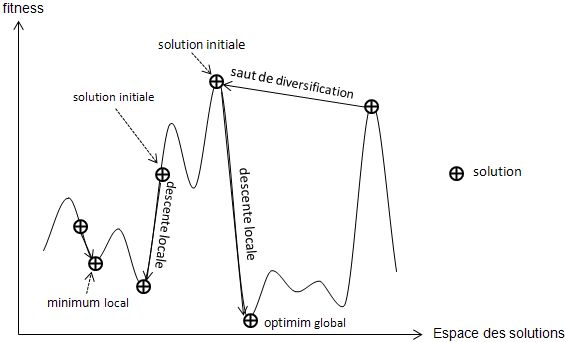
\includegraphics[width=\textwidth]{./Img/principe_ma.jpg}
%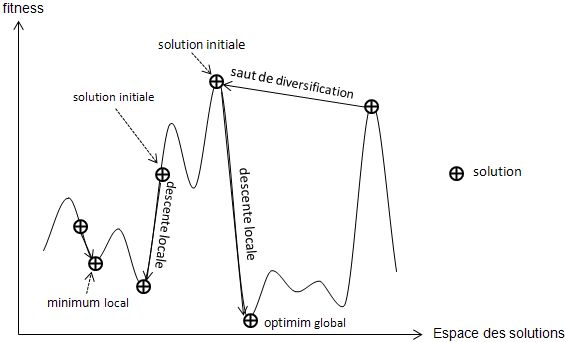
\includegraphics[width=0.75\textwidth, natwidth=510, natheight=542] {./Img/principe_ma.jpg}
\caption{Principe de l'algorithme m�m�tique.}
\label{fig:principe_algo_memetic}
\end{center}
\end{figure}

Des op�rateurs de s�lection permettent le remplacement des \og mauvaises \fg  solutions de la population par les \og meilleures \fg de la population. Un ou plusieurs op�rateurs de mutation participent � la diversification et l'am�lioration des solutions. Il sont mis en \oe{}uvre par les op�rations de base de manipulation des imbrications.

Si nous utilisons une recherche locale au sein d'un l'algorithme �volu\-tionnaire, nous obtenons un algorithme �volutionnaire de type m�m�tique \citep{moscato:03}. La figure \ref{fig:principe_algo_memetic} nous permet de sch�matiser le principe de recherche de solution par l'algorithme m�m�tique. Sur la figure sont illustr�es les recherches locales ex�cut�es en parall�le sur les individus de la population et conduisant � un minimum local. La multiplication de ces recherches locales coupl�e aux op�rateurs de s�lection et de mutation d�termine la dynamique de recherche. L'objectif est de r�utiliser les avantages de la recherche locale tout en fournissant des m�canismes de diversifications pour �viter d'�tre pi�g� dans un minimum local.

\chapter{Structures de donn�es}
\label{chapitre_structures}

L'utilisation de structures de donn�es adapt�es aux proc�dures d'optimi\-sation est un �l�ment cl� du processus de conception. Un des principes cl�s r�side dans l'utilisation de tableaux � acc�s direct indic�s par identifiant.

Nous donnons ci-dessous, une description des �l�ments cl�s de la mod�li\-sation orient�e objet sous forme de diagramme UML. Sont pr�sent�s, les composants de base, les tableaux de donn�es, l'environnement commun d'optimisation.

\section{Structure position}

%\setlength\abovecaptionskip{0cm}

\begin{figure}[h]
 \begin{center}
  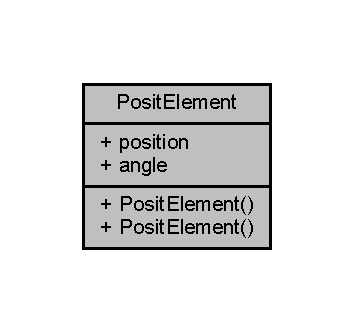
\includegraphics[scale=1]{./Img/struct_posit_element__coll__graph.pdf}
  \caption {Position d'un �l�ment/composant.}
  \label{uml:position}
 \end{center}
\end{figure}

Tout composant g�om�trique est caract�ris� par un point de r�f�rence et un angle d'orientation. Sa position dans le plan est d�termin�e par la position du point de r�f�rence dans le plan et l'angle avec l'horizontale. Le diagramme de classe UML est donn� par la figure \ref{uml:position}.

\section{Objet solution}

\begin{figure}[h]
 \begin{center}
  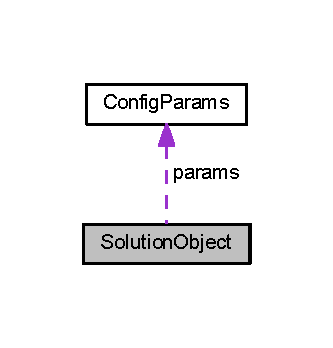
\includegraphics[width=\columnwidth]{./Img/class_solution_object__coll__graph.pdf}
  \caption {Classe principale solution.}
  \label{uml:solution}
 \end{center}
\end{figure}

La classe \textit{SolutionObject} est la structure principale repr�sentant une solution du probl�me. Elle comporte toutes les variables de la solution, variables de positionnement, d'ordonnancement. Chaque solution manipul�e et/ou construite par l'algorithme d'optimisation est une instance de la classe \textit{SolutionObject}. Une solution peut �tre dupliqu�e et reproduite � volont� � l'aide de l'op�rateur d'affectation standard (=). La solution est un objet manipul� par les algorithmes m�taheuristiques de r�solution. Le diagramme de classe UML est donn� par la figure \ref{uml:solution}. Seule la classe de configuration \textit{ConfigParams} apparait ici.



\chapter{Op�rateurs de base}
\label{chapitre_operateurs}

Deux types de m�thodes d'optimisation sont utilis�es. Ce sont respectivement la recherche locale it�r�e et un algorithme m�m�tique dont nous avons donn� les grandes lignes pr�c�demment et que nous d�crivons plus en d�tail dans le chapitre suivant. Ces m�thodes ont en commun un ensemble d'op�rateurs de base op�rant sur la structure d'une solution. 

Dans les deux cas de figure, une ou plusieurs solutions sont modifi�es de mani�re it�rative selon un op�rateur de voisinage qui transforme un ou plusieurs items (�pures) d'une solution courante. Cet op�rateur de voisinage est composite en ce qu'il combine diff�rents op�rateurs de base ayant diff�rentes fonctions (mouvement, swap). L'op�rateur est stochastique en ce que le choix de la modification locale est en partie al�atoire. Plusieurs types d'op�rateurs sont propos�s. Enfin, l'op�rateur de voisinage composite effectue une combinaison probabiliste des op�rations de base.

\section{Op�rateur de mouvement}

\begin{figure}[h]
\centering
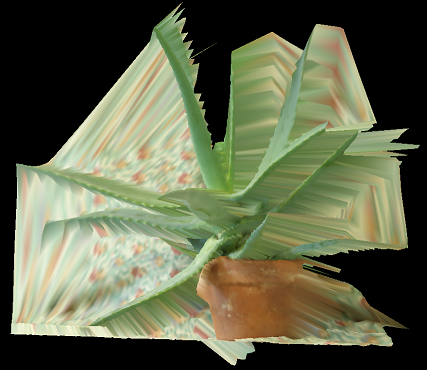
\includegraphics[width=5cm]{./Img/test.png}
\caption{Op�ration de mouvement.}
\label{figure:trans}
\end{figure}

L'op�rateur de mouvement �l�mentaire est illustr� par la figure \ref{figure:trans}. Il permet les op�rations de mouvements. Cet op�rateur de base est appel� par l'op�\-rateur de voisinage composite avec une probabilit� �lev�e (environ 0,9). Il constitue l'op�ration de base la plus active dans le processus d'opti\-misation.

\section{Op�rateur de swap}

\begin{figure}[h]
\centering
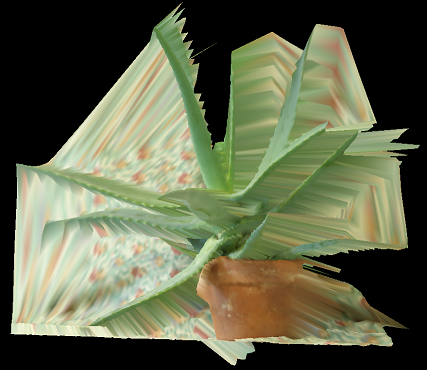
\includegraphics[width=5cm]{./Img/test.png}
\caption{Op�ration de swap.}
\label{figure:swap}
\end{figure}

L'op�rateur de swap est illustr� par la figure \ref{figure:swap}. L'op�ration est appliqu�e par l'op�rateur composite avec une probabilit� assez faible (environ 0,01).

\section{Op�rateur de construction initiale}
\label{const_gloutonne}

\begin{figure}[h]
\centering
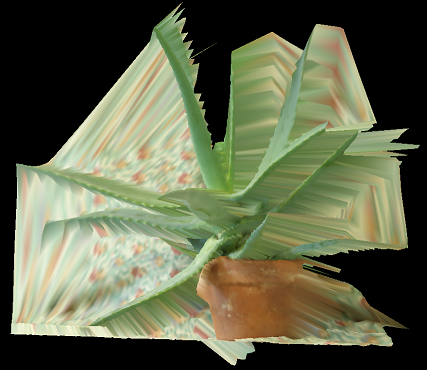
\includegraphics[width=5cm]{./Img/test.png}
\caption{Construction avec bruit al�atoire.}
\label{figure:construction}
\end{figure}

L'op�rateur de construction initiale cherche � produire une solution aussi vite que possible. Le r�sultat n'est pas n�cessairement une solution admissible et peut pr�senter des  contraintes non satisfaites, ainsi qu'illustr� � la figure \ref{figure:construction}. Le pseudo-code est donn� dans l'Algorithme \ref{construct_par}. Noter que l'op�rateur de construction n'est appel� qu'une seule fois pour initialiser une solution. Les recherches locales, et les proc�d�s d'am�lioration m�taheuristiques peuvent alors d�marrer.
%$\rightarrow$  
 
\begin{algorithm}[t] 
\Entree{$S \in$ Solution}
\Sortie{S}
\Deb{
	\tcp{Les composants sont pr�alablement tri�s}
  \Tq{tous les composants ne sont pas plac�s }{
    \Pour{chaque composant $v \in S$}{
	  			Placer le composant selon une strat�gie de construction\;
    }
  }
  \Retour{$S$}\;
}
\caption{Construction initiale (constructSolutionSeq)}
\label{construct_par}
\end{algorithm}

\section{Op�rateur de voisinage}
\label{voisinage}

\begin{algorithm}%[H]
\Entree{$S \in$ Solution}
\Sortie{S}
\Deb{
	\tcp{S�lectionner un des op�rateurs de base selon sa probabilit� d'application}
	\tcp{Appliquer l'op�rateur $i$ s�lectionn� � la solution $S$}
	$S \leftarrow operator_i(S)$\;
	\Retour{$S$}\;
}
\caption{Op�rateur de voisinage composite (generateNeighbor)}
\label{neighbor_operator_0}
\end{algorithm}

L'op�rateur de voisinage composite est utilis� au sein d'une strat�gie de recherche locale ou m�m�tique. Il applique l'ensemble des op�rateurs de base suivant une probabilit� d'ex�cution sp�cifique � l'op�rateur. Noter que l'op�rateur de construction n'est pas concern� puisqu'il fournit seulement la solution de d�part qui va �tre am�lior�e. L'op�rateur de voisinage composite vise � transformer, au pas � pas, une solution non admissible de d�part en une solution admissible avec un co�t le plus r�duit possible en temps d'ex�cution. Son ex�cution inclut la r��valuation incr�mentale de la fonction objectif au sein de chaque op�rateur �l�mentaire, ce qui est crucial pour le temps d'ex�cution. Le pseudo-code est r�sum� par l'Algorithme \ref{neighbor_operator_0}. La fonction de voisinage composite C++ op�rant sur une solution correspond au profil \textit{void SolutionObject::generateNeighbor()}.



\chapter{Algorithme m�taheuristique}
\label{chapitre_6}

Le d�veloppement de m�thodes heuristiques est a priori justifi� par la difficult� du probl�me d'imbrication qui est NP-difficile. Les heuristiques consid�r�es sont trois variantes de recherches locales it�ratives, op�rant sur une solution unique pr�alablement construite mais non n�cessairement admissible, un algorithme �volutionnaire op�rant sur une population de solutions et un algorithme m�m�tique incorporant une recherche locale au sein d'un algorithme �volutionnaire. En d�finitive seuls la recherche locale \textit{First Improvement} et l'algorithme M�m�tique semblent vraiment performant a priori sur un probl�me quelconque. Nous d�taillons cependant les diff�rentes versions.

La recherche locale fonctionne par des mouvements de faible amplitude dans un voisinage de la solution courante. La fonction de voisinage d�termine la solution suivante obtenue � partir d'une modification locale de la solution courante. Lorsqu'aucune am�lioration de la solution ne peut �tre obtenue dans le voisinage, la solution en cours est un optimum local relatif � la fonction de voisinage. La r�it�ration de la recherche locale � partir de conditions de d�part al�atoires permet de diversifier les zones d'exploration.

L'op�rateur de voisinage composite est � la base du principe de la re\-cherche locale. Nous avons retenu trois versions de la re\-cherche locale suivant le mode d'examen du voisinage retenu. La premi�re version est une recherche de type marche al�atoire. Les deux autres versions sont une recherche gloutonne \textit{first improvement search} et une recherche en profondeur \textit{best improvement search}. 

En combinant les m�mes op�rateurs de base dans un sch�ma d'algo\-rithme � base de population, avec des op�rateurs de s�lection sur les solutions, nous sp�cifions un algorithme �volutionnaire. Puis, pour tenter de tirer parti des avantages de l'al\-go\-rithme �volutionnaire et de la recherche locale conjointement, nous incluons celle-ci en tant qu'op�rateur dans un algorithme �volutionnaire selon le principe d'un algorithme m�m�tique.

Dans la section \ref{rech_locale_iteree}, sont pr�sent�es les recherches locales it�r�es selon trois versions. L'algorithme �volutionnaire op�rant sur une population de solutions, et l'algorithme m�m�tique, incluant la recherche locale, sont pr�sent�s dans la section \ref{algorithme_evolutionnaire}.

\section{Recherche locale it�r�e}
\label{rech_locale_iteree}

Les recherches locales combinent les op�rateurs de base selon diff�rentes strat�gies de recherche. Elles op�rent toutes � partir d'une solution unique pr�alablement construite et non n�cessairement admissible. Elles diff�rent par le mode de parcours d'un voisinage autour de la solution courante. Elles sont r�it�r�es avec des ordonnancements de v�hicules modifi�s.

\subsection{Boucle externe}

La recherche locale it�r�e \citep{johnson:97} est l'une des m�thodes les plus simples de recherche heuristique appliqu�es aux probl�mes NP-difficiles. La boucle principale de la m�thode consiste � r�it�rer l'ex�cution de recherches locales simples � partir de conditions initiales al�atoires. Le pseudo-code de la boucle principale est pr�sent� dans l'Algorithme \ref{heur_iter}.

Les op�rations sont reparties en deux phases: une phase de construction suivie d'une phase d'am�lioration. Dans l'Algorithme \ref{heur_iter}, une tentative de construction suivie d'une tentative d'am�lioration sont effectu�es par les deux appels \textit{constructSolution} et \textit{improveSolution}. Les d�tails de ces deux proc�dures sont donn�s respectivement dans les sections \ref{construction_loop} et \ref{local_search_improv}. La construction g�n�re rapidement des solutions partielles non n�cessairement admissibles. A partir de la 
solution obtenue, la proc�dure d'am�lioration applique des modifications locales en vue d'am�liorer la solution.

\begin{algorithm}[htp]
\Sortie{$Best$}
\Deb{
	$S \leftarrow initialize()$;~\tcp{initialisation des structures de donn�es}
	$count \leftarrow 0$\;
	\Tq{$count < maxCount$}{
	  $count \leftarrow count + 1$\;
		$S \leftarrow constructSolution(S)$;~\tcp{construction d'une solution non n�cessairement admissible}
		$S \leftarrow improveSolution(S)$;~\tcp{am�lioration de la solution par recherche locale}
		$Best \leftarrow selectBest(S, Best)$\;
	}
	\Retour{$Best$}\;
}
\caption{Algorithme de recherche locale it�r�e}
\label{heur_iter}
\end{algorithm}

Dans tous les cas de figure, il convient d'�valuer et de comparer des solutions non n�cessairement admissibles. C'est pourquoi, le classement des solutions s'effectue selon la valeur de la fonction objectif agr�gative qui inclut le respect des contraintes. Le d�tail en est donn� dans la section de d�finition du probl�me. Le classement de deux solutions est effectu� par la proc�dure \textit{selectBest}.  

\subsection{Boucle de construction}
\label{construction_loop}

La boucle principale de construction \textit{constructSolution} est d�taill�e dans l'Algorithme \ref{constr_proc}. Son r�le est de g�n�rer aussi rapidement que possible de nouvelles solutions candidates, admissibles ou non, de plus ou moins bonne qualit�. La proc�dure r�p�te \textit{maxConstruct} fois un proc�d� de construction de base. La proc�dure \textit{selectBest} effectue un classement suivant l'objectif global du probl�me.

\begin{algorithm}[t]
\Entree{$S \in$ Solution, $maxConstruct$}
\Sortie{$Best$}
\Deb{
%    $Best \in$ Solution\;
		$count \leftarrow 0$\;
		\Tq{$count < maxConstruct$}{
		  $count \leftarrow count + 1$\;
		  \tcp{Appliquer une op�ration de perturbation}
		  $S \leftarrow perturbationOp(S)$\;
			\tcp{Construction s�quentielle}
			$S \leftarrow constructSolutionSeq(S)$\;
			$Best \leftarrow selectBest(S, Best)$\;
		}
  	\Retour{$Best$}\;
}
\caption{constructSolution}
\label{constr_proc}
\end{algorithm}

\subsection{Boucle d'am�lioration}
\label{local_search_improv}
La g�n�ration de nouvelles solutions de d�part diversifi�es � partir de conditions initiales al�atoires est effectu�e par la boucle de construction. � partir de la solution fournie, l'intensification de la recherche est r�alis�e par la proc�dure \textit{improveSolution} de l'Algorithme \ref{heur_iter} pr�c�dent. Elle permet des mouvements de faible ampleur dans une petite r�gion de l'espace des solutions et tente de transformer des solutions non admissibles en solutions admissibles. Le sch�ma de base d'une proc�dure d'am�lioration consiste � int�grer un op�rateur de voisinage dans une strat�gie de recherche. En suivant ce sch�ma, trois versions de recherche locales sont propos�es : une recherche al�atoire simple et deux recherches locales � pivotage.

\subsubsection{Recherche al�atoire}
La strat�gie de recherche d�finie par l'Algorithme \ref{iter_rand_search} s'inspire du principe de la marche al�atoire. Nous l'avons d�nomm�e recherche al�atoire it�r�e ou IRS. Elle consiste � faire �voluer une solution courante en effectuant un nombre donn� de mouvements successifs dans le voisinage puis � s�lec\-tionner la meilleure solution rencontr�e lors de cette succession de mouvements. La m�thode est tr�s simple car tr�s peu d'op�rations de copie de donn�es sont effectu�es � chaque pas d'it�ration.

\begin{algorithm}[b]
\Entree{$S \in$ Solution, $maxImprove$}
\Sortie{$Best$}
\Deb{
%    $Best \in$ Solution\;
		$count \leftarrow 0$\;
		\Tq{$count < maxImprove$}{
		  $count \leftarrow count + 1$\;
			$S \leftarrow generateNeighbor(S)$\;
			$Best \leftarrow selectBest(S, Best)$\;
		}
  	\Retour{$Best$}\;
}
\caption{iteratedRandomSearch}
\label{iter_rand_search}
\end{algorithm}
\newpage

\subsubsection{Recherche locale}

Dans cette section, nous pr�sentons l'algorithme de recherche locale suivant deux versions. La premi�re est la recherche locale gloutonne, que nous appelons \og recherche locale it�r�e premier meilleur \fg , ou encore ILS-FI. La seconde est la recherche locale en profondeur, que nous appelons \og recherche locale it�r�e meilleure am�lioration \fg , ou encore ILS-BI. L'Algorithme \ref{local_search} donne le code commun aux deux versions. La diff�rence entre les deux ex�cutions tient dans la condition d'�valuation de la boucle interne \og tant que \fg. Le code indiqu� correspond � la version ILS-FI, retenue en d�finitive comme solution performante. L'instruction qui teste la d�tection d'une am�lioration, dans la condition, doit �tre retir�e dans le cas ILS-BI. Par rapport � IRS, ILS-FI et ILS-BI comportent chacune deux boucles imbriqu�es, et non une seule, comme le montre l'Algorithme \ref{local_search}.

\begin{algorithm}[htp]
\Entree{$S \in$ Solution}
\Sortie{$Best$}
\Deb{
%  $Best, S' \in$ Solution\;
	$Best \leftarrow S$\;
  $improvementFound \leftarrow true$\;
	\Tq{$improvementFound~\tcc*[h]{d�finit la profondeur}$} {%\tcp{depth of the search}
 		$count \leftarrow 0$\;
	  $improvementFound \leftarrow false$\;
		\Tq{$count < neighborhoodSize$ {\bf et} $\neg$ improvementFound}{
		  $count \leftarrow count + 1$\;
			$S' \leftarrow generateNeighbor(S)~\tcc*[h]{examen du voisin}$\;
			Si {$isBest(S', Best)$} { 
					$Best \leftarrow S'$\;
  				$improvementFound \leftarrow true$\;
  		}
		}
		$S \leftarrow Best$\;
	}
	\Retour{$Best$}\;
}
\caption{Recherche locale \textit{First Improvement}}
\label{local_search}
\end{algorithm}

La boucle externe contr�le la profondeur de la recherche. L'algorithme s'arr�te lorsqu'aucune am�lioration n'a �t� trouv�e, ce qui correspond � l'atteinte d'un minimum local. La solution courante constitue l'�l�ment pivot autour duquel s'effectue la recherche dans le voisinage. C'est � partir de cet �l�ment que des solutions voisines sont g�n�r�es et examin�es. La boucle interne met en \oe{}uvre la r�gle de pivotage. Elle d�termine la meilleure solution voisine vers laquelle la recherche doit se d�placer. Cette solution devient le nouveau pivot � partir duquel des solutions voisines sont � nouveau g�n�r�es.

Par rapport � la recherche al�atoire it�r�e IRS, nous pouvons noter l'ajout d'une variable suppl�mentaire $S'$ utilis�e pour tester la pr�sence d'une am�lio\-ration. Dans les deux types de recherche locale ILS-FI et ILS-BI, une variable suppl�\-mentaire de m�morisation est donc requise pour tester la possibilit� d'am�lioration, cela entra�ne davantage de copies de donn�es que dans la premi�re m�thode de recherche al�atoire it�r�e IRS.

Dans ILS-FI, la premi�re meilleure solution rencontr�e devient le nouvel �l�ment pivot. Dans ILS-BI, c'est la meilleure solution dans un �chantillon al�atoire du voisinage qui devient le nouvel �l�ment pivot. La taille de l'�chantillon est d�finie par le param�tre \textit{neighborhoodSize} dans l'Algo\-rithme \ref{local_search}. Dans les exp�rimentations, la taille de l'�chan\-tillon peut varier entre 100 et 1000 unit�s examin�es.

\section{Algorithme �volutionnaire et m�m�tique}
\label{algorithme_evolutionnaire}

\subsection{Algorithme}

Suivant la terminologie des algorithmes �volutionnaires, les solutions sont maintenant des \og individus \fg composant une population qui va �voluer de g�n�ration en g�n�ration de mani�re � r�pondre aux exigences du probl�me. Des op�rateurs de variations tels que des mutations vont modifier les individus, ceux-ci �tant soumis � une s�lection suivant leur ad�quation aux objectifs du probl�me.

Ici, nous sp�cifions une boucle prin\-cipale type d�fi\-nissant un algorithme �volutionnaire. Nous pouvons d�cliner cette boucle principale selon un algorithme �volutionnaire classique, mais notre choix apr�s exp�rimentation se porte sur un algorithme de type algorithme m�m�tique. Un algorithme m�m�tique est une extension d'un algorithme g�n�tique, ou �volutionnaire, dans lequel est ajout� une recherche locale en tant qu'op�rateur de modification de solution correspondant � une mutation d'un type particulier \citep{moscato:03}. Nous n'utilisons pas d'op�rateur de croisement. Nous utilisons nos m�thodes de recherche locale et construction en tant qu'op�rateurs de mutation dans la boucle �volutionnaire.

Le pseudo-code de la boucle �volutionnaire type est donn� par l'Algo\-rithme \ref{algo_implant}. Deux op�rateurs de mutations sont sp�cifi�s. Ceux sont les op�\-rateurs \textit{mutate} et \textit{localSearch}. Deux op�rateurs de s�lection au niveau de la popu\-lation peuvent �tre utilis�s. Le premier d'entre eux est l'op�\-rateur appel� \textit{select} dans le pseudo-code. Il remplace $Pop/5$ individus de plus faible \textit{fitness} dans la popu\-lation par $Pop/5$ individus de plus grande \textit{fitness}, avec $Pop$ comme taille de la population d'individus. Le second op�rateur de s�lection et de classement est la version �litiste du premier. Il est appel� \textit{selectElitist}. Il remplace $Pop/10$ individus ayant la \textit{fitness} la plus faible de la popu\-lation, par le meilleur individu $Best1$ rencontr� durant l'ex�cution. En pratique, il s'av�re que la s�lection �litiste n'est pas efficace sur le probl�me. Celle-ci n'est donc pas utilis�e en pratique sur le probl�me.

\begin{algorithm}[htp]
%\KwIn{}
\Sortie{$Best2$}
\Deb{
    $Best1, Best2 \in$ Solution\;
    $P$: Population;\tcp{100 individus}
    $Gen \in$ {\bf Entier}\;
    $Gen \leftarrow 0$\;
    $P \leftarrow generate(P)$; \tcp{G�n�rer les individus} 
    $Best1 \leftarrow getBest(P)$\;
	  \tcp{R�p�ter $MaxGen$ g�n�rations}
    \Tq{$Gen < MaxGen$ {\bf et} $\neg$ (solution construite)}{ 
	  	$Gen \leftarrow Gen + 1$\;

	  	\tcp{Appliquer une op�ration/mutation de voisinage}
	  	$P \leftarrow locaSearch(P)$\;

	  	\tcp{M�moriser le meilleur individu}
		  $Best1 \leftarrow getBest(P, Best1)$\;
		  $Best2 \leftarrow getBest(Best1, Best2)$\;

	  	\tcp{Appliquer les op�rateurs de s�lection}
	  	$P \leftarrow select(P, size(P)/5)$\;
	  	%\tcp{$P \leftarrow selectElitist(P, Best1, size(P)/10)$\;}

		  \tcp{Appliquer une mutation}
		  $P \leftarrow mutate(P)$\;
		  
    }
    \Retour{$Best2$}\;
}
\caption{Boucle type d'un algorithme �volutionnaire}
\label{algo_implant}
\end{algorithm}

\subsection{Version m�m�tique}
\label{algorithme_memetic}

Le d�tail des op�rateurs de mutation pour l'algorithme m�m�tique est donn� dans l'Algorithme \ref{oper_memetique}. Dans ce cas, les op�rations de mutation deviennent des appels aux proc�dures de construction et de recherche locale que nous avons sp�cifi�es ant�\-rieurement. L'op�rateur \textit{mutate} effectue un appel de la proc�dure de construction it�r�e tandis que l'op�rateur \textit{localSearch} ex�cute un appel de la proc�dure de recherche locale. 

L'int�r�t recherch� est de coupler la dynamique de diversi-fication et de s�lection de l'approche �volu\-tionnaire avec des recherches locales adapt�es pour l'intensi\-fication de la recherche dans une zone r�duite de l'espace des solutions. Le principe de l'algorithme �volutionnaire, via une population de solutions et des op�rateurs de s�lection, vise � augmenter la diversit� des solutions potentielles. L'algorithme m�m�tique tire partie des avantages de la recherche locale et de la diversification au sein d'une population.

\begin{algorithm}[htp]
    {Proc�dure \bf generate}{($P \in$ Population)}\\
		\Deb{
	    \Pour{chaque individu $I \in P$} {
				$I \leftarrow constructSolution(I)$ \tcp{Correspond � la construction sp�cifi�e dans l'Algorithme (\ref{constr_proc})}
	    }
	  }
    {Proc�dure \bf mutate}{($P \in$ Population)}\\
		\Deb{
	    \Pour{chaque individu $I \in P$}{
	      \tcp{Appliquer la mutation avec une probabilit� de 0.5}
				\Si{$rand(0, 1) > 0.9$}{	
					$I \leftarrow constructSolution(I)$ \tcp{Correspond � la construction sp�cifi�e dans l'Algorithme (\ref{constr_proc})}
				}
	    }
	  }
    {Proc�dure\bf localSearch}{($P \in$ Population)}\\
	  \Deb{
	     \Pour{chaque individu $I \in P$}{
				$I \leftarrow improveSolution(I)$  \tcp{Correspond � la recherche locale sp�cifi�e � l'Algorithme (\ref{local_search})}
	     }
		} 
\begin{footnotesize}
\begin{tabular}{l}
\end{tabular}
\end{footnotesize}
\caption{Les op�rateurs de variation de l'algorithme m�m�tique}
\label{oper_memetique}
\end{algorithm}


\chapter{Jeux de tests et �valuation}
\label{chapitre_jeux_de_tests}
L'�valuation des heuristiques n�cessite l'utilisation d'instances de probl�me repr�senta\-ti\-ves de la difficult� et de la diversit� des cas r�els d'application. Pour �valuer les m�thodes d'optimisation, sont propos�s un ensemble de jeux de tests, appel�s benchmarks. Chaque dossier de test comporte des instances, issues de cas r�els ou g�n�r�es automatiquement, sur lesquelles sont appliqu�s des sch�mas de r�solution suivant la configuration des para\-m�tres choisis.

Un fichier de configuration type \textit{config.cfg} du programme d'opti\-misation est fourni pour l'ex�cution des jeux de tests. Il d�finit une ex�cution standard avec l'ensemble des fonction\-nalit�s d'optimisation activ�es. Il peut �tre utilis� avec toute instance sans exception, mais peut �tre modifi� ou ajust� suivant la fonction ou l'option que l'on veut utiliser. Les variations des param�tres de configuration pour les diff�rents tests de validation
sont minimes par rapport a la configuration type. Nous d�crivons les sc�narios de tests propos�s en indiquant dans chaque cas les fonctionnalit�s test�es et les changements dans les param�tres de configuration de la configuration type.

Les tests de validation se d�composent en deux groupes, les tests avec g�n�ration d'instances automatique et les tests avec instances issues de cas r�els ou instances sp�cifiques. Ils sont pr�sent�s ci-apr�s avec des exemples de r�sultats. Noter qu'il est possible de lancer une ex�cution compl�te automatis�e de tous les tests � l'aide de scripts syst�mes d'ex�cution tels que la commande \textit{./test/test\_all.bat}.

Les dossiers de tests avec g�n�ration automatique d'instances sont les suivants :
\begin{itemize}
\item     \textit{test exemple type avec g�n�ration automatique}
\end{itemize} 

Les dossiers de tests portant sur des instances issues de cas r�els sont les suivants :
\begin{itemize}
\item     \textit{test exemple type}
\end{itemize} 

\section{Crit�res d'�valuation}

Les valeurs des crit�res d'�valuation d'une solution sont renvoy�es dans le fichier \textit{output.stats}. Ils correspondent presque exactement aux objectifs du probl�me. Nous distinguons les objectifs des crit�res dans la mesure ou les premiers renvoient � la repr�\-sentation interne de l'�valuation de la solution et les seconds renvoient aux valeurs pr�sent�es � l'uti\-lisateur ext�rieur. Les cri\-t�res correspondent aux objec\-tifs, except� qu'il peuvent �tre plus nombreux et compl�mentaires.

Les crit�res d'�valuation d'une solution renvoy�s dans le fichier \textit{output.stats} sont les suivants :

\begin{itemize}

\item \textit{iteration} : num�ro d'it�ration lors de l'�valuation
\item \textit{f\_objectif\_1} : premier objectif
\item \textit{f\_objectif\_2} : second objectif
\item \textit{f\_objectif\_3} : troisi�me objectif
\item \textit{duree}(s) : dur�e d'ex�cution en secondes
\item \textit{duree}(s.xx) : dur�e d'ex�cution en secondes et millisecondes

\end{itemize} 

Noter que chaque r�pertoire de test comporte un fichier Excel pour l'analyse statistique des r�sultats de nom \textit{result\_analysis.xlsx}. Il est ainsi possible d'�valuer rapidement les performances moyennes de l'algorithme relativement � un grand nombre d'ex�cutions.

\section{Test standard avec g�n�ration automatique}

Il s'agit de tester des fonctionnalit�s sur des jeux de tests g�n�r�s automatiquement � partir d'un mod�le. Le test permet aussi d'illustrer la post-optimisation. Pour dissocier des fonctions, on utilise dans ce test un mode "post-optimisation" qui applique une nouvelle fonction, ou configuration, sur la solution pr�c�demment obtenue. Pour configurer l'application en mode post-optimisation, il suffit de sp�cifier les param�tres suivants :
\begin{itemize}
\item  $constructFromScratchParam = false$
\item  $MAnbOfInternalConstructs = 0$ 
\end{itemize} 

Le principe du test consiste � lancer une premi�re phase d'optimisation avec des param�tres actifs et ensuite � lancer une post-optimisation en retirant l'option en question. L'ajout ou suppression des fonctions peut �galement �tre r�alis� via les poids des objectifs. Les param�tres de confi\-guration de d�part sont les suivants :

\begin{itemize}
\item $utiliseFonction = true$
\end{itemize}

\begin{figure}[h]
\centering
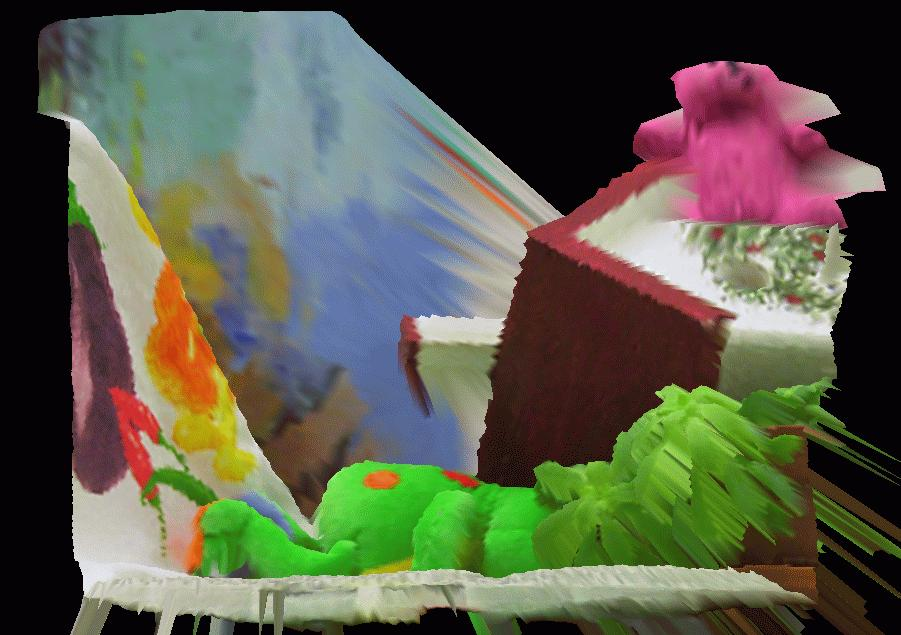
\includegraphics[width=\columnwidth]{./Img/test.jpg}
\caption{Solution type.}
\label{figure:reptr}
\end{figure}

Un exemple de r�sultat est visualis� � la figure \ref{figure:reptr}. On constate que les contraintes sont satisfaites. La solution est admissible sur l'ensemble des crit�res.

\section{Test standard cas r�el}

Il s'agit d'un test issu de cas r�els consid�r� difficile � r�soudre. Il est r�solu en moins de 0.1 secondes sur un PC Dual Core avec GPU. Dans ce cas difficile, pour acc�l�rer au maximum la vitesse de r�solution, il convient d'inhiber l'activation de certaines fonctions. Ces fonctions peuvent �tre inhib�es avec les commandes :
\begin{itemize}
\item $utiliseFontion\_1 = false$
\item $utiliseFonction\_2 = false$
\end{itemize} 

Une solution est repr�sent�e � la figure \ref{figure:test}.

\begin{figure}[h]
\centering
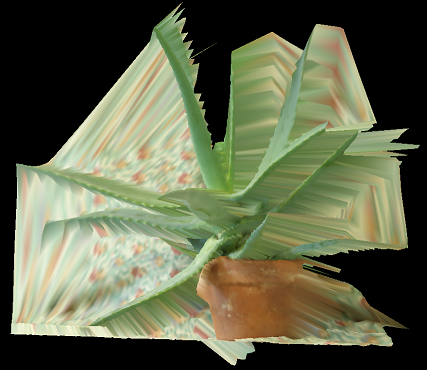
\includegraphics[width=\columnwidth]{./Img/test.png}
\caption{Solution type.}
\label{figure:test}
\end{figure}


%\include{./Chapters/chapitre_evaluation}
\chapter*{Conclusion}
\label{conlusion_generale}
\addcontentsline{toc}{chapter}{Conclusion}
\markboth{Conclusion}{Conclusion}

L'objectif de ce document �tait de pr�senter les principes de la conception des algorithmes d'optimisation pour un probl�me type. Nous retenons en d�finitive deux approches d'optimisation efficaces sur le probl�me, la recherche locale \textit{First Improvement}, et l'algorithme M�m�tique.



%------------------------------------------------------------------------------------------------------
%  Annexes
%\appendix
%\input{./annexes/A/annexeA.tex}
%\chapter*{Glossaire}
\addcontentsline{toc}{chapter}{Glossaire}
\markboth{Glossaire}{Glossaire}
\begin{quote}
  Les abr\'eviations et acronymes pr\'esents dans ce glossaire sont signal\'es dans le texte par un ast\'erisque ($^\ast$).
\end{quote}

\begin{description}
  \item[ACG] Application Communication Graph
  \item[BE] Best Effort
  \item[CDG] Communication Dependency Graph
  \item[CKPP] Cyclic $K$-conflict-free shortest Paths Problem
  \item[CPU] Central Processing Unit
  \item[CRKPP] Cyclic Reconfigurable $K$-conflict-free shortest Paths Problem
  \item[DSP] Digitial Signal Processor
  \item[EDP] $K$-Edge-Disjoint Shortest Paths Problem 
  \item[FPGA] Field-Programmable Gate Array
  \item [GLPK] GNU Linear Programming Kit
  \item[GT] Guaranteed Traffic
  \item[ILP] Integer Linear Program
  \item[ILS-BI] Iterated Local Search - Best Improvement
  \item[ILS-FI] Iterated Local Search - First Improvement
  \item[IP] Intellectual Property
  \item[IRS] Iterated Random Search
  \item[MCU] Micro Controller Unit
  \item[MPSoC] multi-processor System-on-chip
  \item[MRT] Maximum Reception Throughput
  \item[NI] Network Interface
  \item[NoC] Network on Chip
  \item[OS] Operating System
  \item[OSI] Open Systems Interconnection
  \item[QAP] Quadratic Assigment Problem
  \item[QoS] Quality of Service
  \item[RTIP] Reconfigurable Traffic Injection Problem
  \item[SoC] System on Chip
  \item[TDMA] Time Division Multiple Access
  \item[TEG] Time-expanded graph
  \item[TIP] Traffic Injection Problem
  \item[TSL] Traffic Saturation Level
  \item[UFP] Unsplittable Flow Problem
\end{description}


%------------------------------------------------------------------------------------------------------
%  Biblio
%\nocite{*}
\bibliographystyle{plain}%{alpha}
%\bibliographystyle{unsrtnat.bst}%{alpha}
\bibliography{./Biblio/biblio}
%\addcontentsline{toc}{chapter}{References}


\end{document}

